\setcounter{chapter}{4}
\chapter{Modelling}
\label{chap:modelling}
% 
\markus{This is an example.}
% 
\section{Introduction}
% 
Nerve fiber modelling is a unique technique often used in simulations like \ac{dMRI}-simulations \dummy.
However, most \ac{dMRI} simulation tools use fast numeric simulation techniques like \dummy.
These use analytical functions to describe the fiber paths in order to calculate very quickly and accurately.
Current algorithms are able to use spline functions for single nerve fibers or fiber bundles \cite{Balls2009}.
Recently, with the improvement of computer performance and algorithms, simulation techniques such as Monte Carlo \dummy are used.
These simulate the random movement of individual water molecules within a volume.
If the target are \ac{WM} phantoms nerve fibers can be modelled as a meshed tube.
If \ac{WM} phantoms are involved, nerve fibers can be modeled as a meshed tube.
These have the advantage that any complex configuration can be modeled \eg fibers \dummy.
\\
%
A disadvantage, however, is that realistic model sizes require individual nerve fiber models in the order of \SI{1}{\micro\meter}.
Experimental \ac{dMRI} system have voxel sizes in the range of \SIrange{100}{1000}{\micro\meter}.
This means that for a signal the number of triangles in the mesh is quite large [\dummy].
Another challenge is to build a geometric configuration where no nerve fibers overlap (\ie, take the same volume in space).
\\
% 
Collision detection plays an important role in this process.
While other simulations that use geometric models (\eg protein folding \dummy) may use something like electric potentials where the actual geometric boundary is not so important.
In the case of \ac{3D-PLI} (and \ac{dMRI}) it will be shown to be different.
\\[\baselineskip]
% 
The following procedures are described in this chapter:
\begin{itemize}[nosep]
    \item geometric representation of the nerve fiber (bundle)
    \item user-friendly construction methods of models
    \item how to ensure collision-free models
\end{itemize}
% 
All described methods can be used within the package \pymodule{fastpli.model}:
% 
\begin{itemize}[nosep]
    \item \pymodule{sandbox}
    \item \pymodule{solver}
\end{itemize}
% 
The first module \pymodule{sandbox} contains routines that help the user to create simple geometric configurations.
These can then be used to build more complex structures of nerve fiber bundles.
The second module \pymodule{solver} contains a \CXX framework wrapped in a \python class to allow the user to build simpler \ac{API} (see \dummy).
\\
% 
First, however, it must be decided how a nerve fiber and a nerve bundle is to be represented.
% 
% 
% 
\section{Nerve fiber representation}
\label{sec:nerve_fiber_representation}
% 
As described in \cref{sec:fiberArchitecture} \ac{WM} consist of densely packed bundles of nerve fibers.
Nerve fibers in \ac{WM} consist of axons surrounded by myelin (see \cref{fig:nerveFiber}).
The myelin is further split into several parts separated by Ranvier nodes to allow the spread of an action potential.
In the central nervous system, myelin is produced by olegodendrocytes, i.e. cells that wrap their small \say{arms} around locally adjacent axons.
The wrapping substance is called myelin and consists mainly of a lipid (fat) substance.
The question is how this tissue can be modelled and represented.
\\
% 
The main focus of modeling is to ensure that these models can be used for \ac{3D-PLI} simulations.
However, it is reasonable that these models can also be used for other tasks \eg for \ac{dMRI} simulations.
% 
\paragraph{What means usable?}
Since simulations are used, computer algorithms must be able to receive an input for a geometric fiber architecture.
One possibility is to look into the field of visualization techniques.
There, objects of different shapes have to be represented so that the computer algorithm can use the representation to visualize an image of the objects.
An obvious model for a fiber is a tube.
Usually objects like tubes are visualized with a surrounding mesh.
Meshes have the advantage that a texture can be applied to the surface.
However, since meshes usually consist of 3D triangles, this means a lot of points, \ie data and memory, for a good approximation to represent a model.
But even in the visualization domain tubes are not modeled from initial meshes.
They are initialized by a trajectory, which is then given an additional radius to obtain a volumetric representation.
This representation can also be used for nerve fiber tissue.
\\
% 
Existing simulation techniques \dummy allow to represent such structures as analytical mathematical objects \eg a parametric function $f(t) -> (x,y,z,r)$ with $(x,y,z)$ as 3D coordinate and $r$ as radius.
However, this drastically restricts the use of this function, since the user needs to know a parametric function in advance.
For trivial structures such as parallel straight fibers this is quite easy and fast to process.
However, if we want to model more complicated fabrics like densely interwoven fiber bundles, the task is almost impossible.
One possibility would be not to care if two fibers overlap, \ie occupy the same space in the volume.
This is done \eg for simulations such as protein folding, where the main interaction comes from electrodynamic forces.
However, it has already been shown that for more complicated \ac{3D-PLI} Simulations non-overlapping fibers are essential [\dummy].
\\
% 
For this reason, it was decided to represent fibers in such a way that they can be easily checked later whether colliding objects, \ie nerve fibers, are present.
\\
% 
\begin{figure}[!t]
    \centering
    \setlength{\tikzwidth}{0.75\textwidth}
    \inputtikz{gfx/model/conical_capsule_bb}
    \tikzset{external/export=false}
	\caption[cc and co]{\Acf{CC}: \raisebox{.25em}{\tikz \draw[black](0,0)--(0.275,0);} \ac{CC}, \raisebox{.25em}{\tikz \draw[blue, dash pattern=on 2.5pt off 2.5pt](0,0)--(0.275,0);} capsule, \raisebox{.25em}{\tikz \draw[red, dash pattern={on 2.5pt off 0.9pt on 0.42pt off 0.9pt}](0,0)--(0.275,0);} bounding box}
	\label{fig:conical_capsule}
\end{figure}
% 
\begin{figure}[!t]
    \centering
    \setlength{\tikzwidth}{0.5\textwidth}
    \inputtikz{gfx/model/capsule}
	\caption{schematic capsule}
	\label{fig:conical}
\end{figure}
% 
In order to enable any level of detail, a tubular fiber can be divided into a number of segments.
Each tubular segment can then be approximated as a cylindrical object.
However, since the radius of the nerve fibers can vary quite a lot along their path, the tube (or the fiber segments) must also be allowed to change.
If this is done via a cylindrical approximation, the boundary effects between two segments can lead to an unusual appearance/behavior.
It was therefore decided to approximate a fiber segment with a \ac{CC}, a 3D cone on which end spheres with the required radii are attached (see \cref{fig:conical_capsule}).
This has the advantage that between two fiber segments there is a smooth transition along the fiber axis (for reasonable curvature) (see \cref{fig:fiberReb, fig:model_length}).
% 
\begin{figure}[!t]
    \setlength{\tikzwidth}{0.85\textwidth}
    \centering
    % \tikzset{external/export next=false}
    \inputtikz{gfx/model/fiber_model}
	\caption[]{Representation of a nerve fiber from a list of spheres.}
	\label{fig:fiberReb}
\end{figure}
% 
A nerve fiber can therefore be represented as a list of 4d coordinates (or spheres) (see \cref{fig:fiberReb}):
% z
\begin{align}
\begin{split}
% \vv{p} &= (x_i,y_i,z_i) \mid x,y,z \in \mathbb{R}\\
% r &\mid r \in \mathbb{R}\\
\mathit{fiber} &= \left\{ \vv{p}_i=(x_i,y_i,z_i), r_i \mid x,y,z \in \mathbb{R}, \, r \in \mathbb{R^+}, \, i \in \{0,1,...,N_{\mathit{points}}-1\}\right\} \\
\mathit{fiber\_segment}_i &= (\vv{p}_i, \vv{p}_{i+1}, r_i, r_{i+1}), \, i \in \{0,1,...,N_{\mathit{points}}-2\}
\end{split}
\end{align}
% 
\section{Sandbox}
% 
Since the geometric representation of the fibers is defined, the question arises how such fibers can be constructed.
For this purpose the \ac{fastPLI} module \textit{fastpli.model.sandbox} was developed.
It contains a variate of methods to allow the user fast building algorithms to generate complex phantoms.
\\
% 
These Algorithms can be split into two parts.
Since this toolbox concentraits to prepair phantoms for the \ac{WM}, the focus on building also n buolding such structures.
Since \ac{WM} nerve fiber bundles are usually combined into nerve fiber bundles (see \dummy), the \textit{sandbox} module contains two major parts o buld exatly such structures.
%
Nerve fiber bundles can be represented in a similar way as nerve fibers: tube like structures populated with individual nerve fibers.
How to represent tube structures was already accomplished (see \cref{sec:nerve_fiber_representation}).
\\
If we think of nerve fiber bundles as a trajectory through the 3d coordinate systems, we can use the same representation as of nerve fibers.
Additionally the contained radii can be used to scale a nerve fiber along its trajectory, \ie to inflate it.
\\
% 
The question remains, how to \say{populate} such bundles.
To populate a trajectory we can use a similar approach to tractography (see \cref{sec:fillBundle}).
We start with seed points at the beginning of the bundle.
\todo{improve transition}
% 
\subsection{Seeding a nerve fiber bundle}\label{sec:seeds}
% 
\begin{figure}[!t]
    \def\tikzheight{0.25\textwidth}
    \centering
    \subcaptionbox{\label{fig:triGrid}equilateral triangle grid}[.295\textwidth]{
    \inputtikz{gfx/model/triangular_grid}\hfill}
    \subcaptionbox{\label{fig:rndGrid}random grid}[.295\textwidth]{
    \inputtikz{gfx/model/rnd_circle_points}}\hfill
    \subcaptionbox{\label{fig:crossBundle}populated fiber bundles}[.39\textwidth]{
    \inputtikz{gfx/model/crossing_bundle}\hfill}
	\caption{Populating fiber bundles with seed points.}
% 	\label{fig:}
\end{figure}
% 
The initial seed can already determine specific outcomes of nerve fiber bundle geometries. 
They are stored as a list of 3d points:
\begin{align}
\mathit{seeds} = \left\{ \vv{p}_i=(x_i,y_i,z_i) \mid x,y,z \in \mathbb{R} , \, i \in \{0,1,N_{\mathit{seed\_points}}-1\}\right\}
\end{align}
% 
To build escepcially dense fiber bundles, a method to generate a equiliteral triangular grid was implemented.
Mathematically a 2d packed circle contains the maximum package density if it is arrange in a triangular (or sometimes called hexagonal) grid for circles with equal radii (see \ref{fig:triGrid}).
This highly regular symmetrical grid can however lead later to strange results in simulations (\eg maxwell, simpli).
\todo{why rnd necesarry -> see simulation}
Therefore it should only be uses as a initial configuration. 
The positions can easily modified.
A useful method was to add a rand value to the initial seed points, \eg $\mathit{shift} = norm(0,\sigma)$.
However since the initial configuration is often unknown, it would be probably best to choose a random distribution.
For a circle this is done via:
\begin{equation}
\begin{aligned}
 \varphi &= \mathrm{uniform}(0,2 \pi) \hspace{4.2ex} && x = r \cos(\varphi)\\
 r &= R \sqrt{\mathrm{uniform}(0,1)} && y = r \sin(\varphi)
\end{aligned}
\end{equation}
% 
\subsection{Populate bundles}\label{sec:fillBundle}
% 
\begin{figure}[!t]
    \centering
    \subcaptionbox{\label{fig:torsionCurve}Torsion along trajectory. The 
	\textcolor{green!50!black}{binormal}, \textcolor{red}{principal normal} vector and \textcolor{blue}{tangent vector} vector at each step are also the coordinate system for the seed points.}[.5\textwidth-4.3pt]{
    \setlength{\tikzwidth}{0.5\textwidth - 4.3pt}
    \inputtikz{gfx/model/min_torsion}}\hfill
    % 
    \subcaptionbox{\label{fig:filledBundle}Bending fiber along trajectory $f(t) = \left(\cos(t), \sin(t), 0 \right)$}[.5\textwidth-4.3pt]{
    \resizebox{.5\textwidth-4.3pt}{!}{
    \includegraphics{dev/gfx/circle_bundle.png}}}
	\caption{}
% 	\label{fig:}
\end{figure}
% 
To populate a nerve fiber bundle, the same idea as in tractography is used.
There, seed points are initialized, and then via \dummy methods a next step is calcuulated.
However, we don't need to calculate the next step, sinice it is already defined by its trajectory.
However, the bending of the bundle has to be taken into account.\\
% 
Here, different techniques already exists.
A common one is to use the torsion of the curve. This is achieved via the following method:
% 
\begin{align}
\begin{split}
\vv{f}(s) &= (x(s),y(s),z(s)) \\
\vv{t}(s) &= \vv{f}\,'(s) \\
\vv{n}(s) &= \frac{\vv{t}\,'(s)}{|\vv{t}\,'(s)|} = \frac{\vv{r}\,''(s)}{|\vv{r}\,''(s)|} \\
\vv{b}(s) &= \vv{t}(s) \times \vv{n}(s),
\end{split}
\end{align}
% 
where $\vv{f}(s)$ is a parameterised trajectory of the parametric variable $s$, $\vv{t}(s)$ the tangential vector, $\vv{n}(s)$ the principal normal vector and $\vv{b}(s)$ the binormal vector (see \cref{fig:torsionCurve}).
One could use this idea to rotate the seed points into the coordinate system of $\vv{t}(s),\vv{n}(s),\vv{b}(s)$.
However this can lead to a arbitry rotation of the fibers, \eg when the curve descibes such a way that $\vv{n}(s),\vv{b}(s)$ would continous rotating around $\vv{t}(s)$.
\\
% 
Since it is plausible, that nerve fiber bundles would not do this, a different approach was decided.
The idea is, to minimise the rotation from one step to the next step.
% If the trajectory, \ie nerve fiber bundle is at step $i$, it came form $i-1$ and goes to $i+1$.
% Therefore one can describe a perpendicular plane between this points:
If we define a plane, inside the above define vectors $\vv{n}(s),\vv{b}(s)$ we want that from one step $i$ to the next step $i+1$ the plane is rotated by the same amount as the curve bends.
However the rotation along the vector $\vv{t}(s)$ shell be $0$.
Since we have a discrete points, we can therefore rotate the plane with the same amount, as the vector $\vv{t}(s)$ obtains.
However to optain a plane in the \say{middle} of the points $\vv{p}_{i-1}, \vv{p}_{i}, \vv{p}_{i+1}$ we will use the mean orientation of these points.
An example is shown in \cref{fig:filledBundle}.
\\
\todo{explain and check algorithm}
% 
Now the populate of the bundle can simply full filled by starting a the beginning of the fiber, placing the seed points at the start point, and rotating the seed point for each step $i$ along the trajectory by only rotating along one vector perpendicular to the curve bending.
% 
\subsection{cube models}
% 
\begin{figure}[!t]
    \centering
    \setlength{\tikzwidth}{0.5\textwidth}
    \inputtikz{gfx/model/cube_build}
	\caption{Populating a cuboid with straight fibers initialized from seed points along the direction $\vv{v}$.}
    \label{fig:cubeBuild}%
\end{figure}
% 
To be able to generate a model with a main fiber orientation, a method to populte a cuboid volume was developed as well.
This method allows to generate fibers inside the cuboid volume which are orientated along a user given main orientation $\vv{v}$ (see \cref{fig:cubeBuild}). 
The individual fibers are initialized with seed points as well.
A infinity line will be placed through each seed point with the main orientation $\vv{v}$.
If a line is colliding with the volume, the line inside the cuboid is returned as a fiber.
% 
\subsection{cylindric models}
% 
\begin{figure}[!t]
    \centering
    \setlength{\tikzwidth}{0.31\textwidth}
    \subcaptionbox{\label{fig:cylCircular}%
        \dummy.
    }[.33\textwidth-1ex]{
    \inputtikz{gfx/model/cylinder_circular}}\hfill
    % 
    \subcaptionbox{\label{fig:cylRadial}%
        \dummy.
    }[.33\textwidth-1ex]{
    \inputtikz{gfx/model/cylinder_radial}}\hfill
    % 
    \subcaptionbox{\label{fig:cylParallel}%
        \dummy.
    }[.33\textwidth-1ex]{
    \inputtikz{gfx/model/cylinder_parallel}}
	\caption{The green area indicates the surface corresponding to the seed points xy-plane. The \textcolor{red}{red} coordinate system indicates the coordinates origin for the seed points.}
% 	\label{fig:}
\end{figure}
% 
Finally a method to build cylindrical structures was implemented as well.
Since a cylinder has three symmetries, all three were implemented to be a option to populate the volume.
First we define the coordinate system.
The cylinder of an outer radii $r_{\mathit{out}}$ and inner radii $r_{\mathit{in}}$ will be orientated along the z-axis with a height $h$, starting at $(0,0,0)$.
Additionally the cylinder can be radial be \say{cut} from a directional angle $\alpha$ to $\beta$.
% 
\paragraph{a) circular} mimics a path on the $xy$-plane of a cylinder (see \cref{fig:cylCircular}).
The seed points will be used along the surface of cross section beginning at the first directional angle $\alpha$.
From there the fibers path will go along circular until the second directional angle $\beta$.
The step size of the circular path can be changed.
% 
\paragraph{b) radial} cylindric fibers are orientated from the center of the $xy$-plane the outside of the cylinder (see \cref{fig:cylRadial}).
The seed points are localized along the inner radial plane.
This way the fiber density will decrease along their path.
% 
\paragraph{c) parallel} fibers are orientated along the cylinder (see \cref{fig:cylParallel}).
Here the seed points are in the $xy$-plane. Only fibers will be used, which are colliding with the cylinder.
% 
\section{Solving fiber collisions/Solver module}
\label{sec:Solver}
% 
One major drawback of all previous methods is, that the user has to make sure, that his fiber trajectory let enough space, so that the fibers (trajectories + radii) have enough space and do not intersect with each other.
This maybe achievable for fibers with constant radii along there path for the upper construction methods.
However, for more slightly more complex structures, \eg crossing fiber bundles, this already is nearly impossible.
Therefore a method was developed, which takes the user defined fibers and checks them for collisions.
When a collision is found it will try to move the colliding objects slightly apart, so that the collision will start to disappear.
\\
% 
This concept is rather simple.
The algorithm for collision detection are already used for century's especially in gaming world, where a character \eg should not be capable to walk through a wall. Another wide verity of algorithms are used in visualisation. There usually the problem is to detect the collision between a light path (mathematical line) and a object, usually a triangular surface. Also known as ray tracing.
The drawback in both fields is, that computing time is limited.
Therefore there algorithms use shortcuts as close to reality as possible but still produce usable data. \eg in computer games it is very important to have a stable frame rate of above $\num{60}$ \ac{fps} (or with the current technology even above 120 \ac{fps}).
However it does not matter much for the gaming experience, if the character can walk slightly into a object or not.
Therefore an object like a stone could be approximated by a sphere(s).
\\
%
However since here we want to generate as good as possible large, complex and precise models, a new algorithm has to be developed which is specialised in this subject.
% 
\\[\baselineskip]
%
\section{World/main}
% 
\begin{lstfloat}[!tb]
\lstset{style=python}
\begin{lstlisting}[]
def step():
    # Reset Parameter
    SetSpeed(objects, 0)
    
    # Building Octree
    octree = Octree(objects)
    
    # Collision Detection
    for leaf in octree:
        colliding_objs = CheckLeaf(leaf.fiber_list)
        colliding_list.insert(colliding_objs)
	
    # Seperation Process
    AddSpeed(colliding_list)
    NormalizeSpeed(colliding_list)
    MoveObject(colliding_list)
	
    # Shape Control
    SegmentLength(colliding_list, target_length)
    BendingRadius(colliding_list, target_curvature)

    return colliding_list.is_empty()
\end{lstlisting}
\caption{Pseudocode of the main algorithm: The function \texttt{FiberCollisionSolver} will loop the followings four steps, which are run in parallel, until no collision are detected anymore: 1. build an \texttt{octree} from all objects, 2. \texttt{Collision Detection}, 3. \texttt{Seperation Process} and 4. \texttt{Shape Control}. \todo{check algorithm, spetially movement phase}}
\label{alg:pseudocode_solver}
\end{lstfloat}
% 
The world/main function is the \say{loop} which is executed to calculate for e collision, moving the objects, and checking the boundary collision (see \cref{alg:pseudocode_solver}).
The looping procedure is similar to a game loop or visualisation loop (\eg opengl main loop).
However, to allow the user as much control as possible, the user has to loop over each step in thir own loop, or use one of the examples inside the packages.
After each step the user is now capable to change parameter, fiber trajectories, add/rm fibers from the \say{scene}, and so on.
Additionally the user can decide, if a fully solved volume is necesarry and for example break out of the solving loop before this step. 
\footnote{Later this behaviour will be researched}
%
\comment{
For this purpose an algorithm was developed and publish in \cite{matuschke2019}.
It is at this point integrated inside the \ac{fastPLI} package under \pymodule{fastpli.model.solver}.
It structure consist out of the following parts:
\begin{itemize}[nosep]
\item main loop
\begin{itemize}[nosep]
    \item octree separation
    \item collision detection
\end{itemize}
\item moving objects
\item apply boundary conditions
\end{itemize}
% 
Before we go into the details of the algorithm, first we descipe the collision detection approuch.
}
\subsection{Collision Detection}
% 
% 
\begin{lstfloat}[!t]
\resizebox{\textwidth}{!}{
% \begin{sideways}
\begin{tabular}{|cc|cc|}
\hline
\hspace{1em} &
\begin{minipage}{0.4625\textwidth}
\lstinputlisting[style=cpp,basicstyle=\scriptsize\ttfamily,firstline=1,lastline=32]{code/collision_detection.py}
\end{minipage} & \hspace{1em} &
\begin{minipage}{0.4625\textwidth}
\lstinputlisting[style=cpp,basicstyle=\scriptsize\ttfamily,firstline=33,lastline=64,firstnumber=35]{code/collision_detection.py}
\end{minipage} \\
\hline
\end{tabular}
% \end{sideways}
}
\caption{Collision detection between two capsule objects. The distance as well as the points on the line segments is returned. A collision takes place if the distance is smaller than $\mathit{cone_a.r}+\mathit{cone_b.r} > d$.}
\label{pseudocodeCollisionDetection}
\end{lstfloat}
% 
As it was described in \cref{sec:nerve_fiber_representation} nerve fibers are represent as a chain of spheres, where two neighbouring spheres are combined into a fiber segment forming a \ac{CC} (see \cref{fig:conical_capsule}).
% 
Therefore an algorithm is necessary to calculate a collision between to \ac{CC}.
This is a non trivial task and very computational heavy.
Therefore it was decided to change the object representation for the collision detection part from a \ac{CC} to a Capsule (see \cref{fig:conical_capsule}).
This means, that the radii of the \ac{CC} grows for both spheres to the max of both spheres $r_{\mathit{capsule}} = \mathrm{max}(r_0, r_1)$.
This has the disadvantage, that at intersections between two neighbouring cones the radii can be actually smaller, however if the change in radii is not rapid, it is justifiable.
\\
The algorithm to detect collisions between two capsules is shown in \cref{alg:pseudocodeCollisionDetection}\footnote{\href{https://www.john.geek.nz/2009/03/code-shortest-distance-between-any-two-line-segments/}{https://www.john.geek.nz/2009/03/code-shortest-distance-between-any-two-line-segments/}}.
% 
It works on the principle, that it calculates the shortest distance between two line segments.
Three cases can occur.
First, the shortest distance is a line perpendicular two both line segments of the cones.
Second, only one line segment is perpendicular to the shortest distance line.
The other has an anchor point at either his first or second point.
Third, the shortest distance is a connection between one of the point of both cones.
For cones a collision is present if the distance is smaller than the sum of both radii.
\\
\begin{figure}[!t]
    \centering
    \def\tikzheight{0.5\textwidth}
    \inputtikz{gfx/model/shortest_dist}
	\caption{shortest distance}
	\label{fig:shortDist}
\end{figure}
% 
The Problem occurring with \ac{CC} is, that since the radii changes along its axis, it is not simply the case anymore, that the shortest distance between two line segments is also the shortest distance between a 3d \ac{CC}.
% 
The calculation of the collision check is expected to be the most costly function at this point.
Therefore the next logical step is to reduce the amount of calculations as far as possible.
A first bruteforce collision check would check each object with all remaining objects.
The next object has then to be checkt with $n-1$ and so on.
This leads to a computational cost of $\mathcal{O}(n^{2})$ which is for large n not acceptable.
To reduce the amount of collision checks have to be done an octree structure is used.
% 
\subsection{octree}
% 
\begin{figure}[!t]
    \centering
    \subcaptionbox{\label{fig:octreeCube}octree}[.3\textwidth]{
    \def\tikzheight{0.6\textwidth}
    \inputtikz{gfx/model/oct_tree}}
    \subcaptionbox{\label{fig:collision2D}collision 2d}[.65\textwidth]{
    \def\tikzheight{0.6\textwidth}
    \inputtikz{gfx/model/collision_tree}}
	\caption{}
	\label{fig:octree}
\end{figure}
% 
A \say{tree} is a data structure consist of a collection of \say{nodes}, which are connected to each other.
One node is conected toward the \say{root} with a single parent node and towards the \say{branches} with several \say{children} or \say{branches}.
The nodes at the end of a branch are refered to as \say{leafs} wich contain the data.
Traversing a evenly distributed tree has the advantage of beeing of computational cost of $\mathcal{O}(\log(n))$.
\\
% 
An octree is a special kind of tree where each node contain 8 children.
This allows to divide \ie a cubic volume into eight equal cutted subcubes.
An example is shown in \cref{fig:octreeCube}.
This means that the length of the volumes shrink exponentialy with $(1/2)^\mathit{level}$.
% 
An octree can be implemented in different ways.
Here a recursion function was chosen (see \cref{alg:pseudocode_octree}).
% 
\begin{lstfloat}[!tb]
\lstset{style=python}
\begin{lstlisting}[]
def octree(volume, objects):
    if num(objects) > threshold:
        sub_volumes, sub_objects = split(volume, objects)
        leafs = [octree(v,o) for v,o in zip(sub_volumes, sub_objets)]
    else:
        leafs=[objects]
    return leafs
\end{lstlisting}
\caption{Pseudocode of octree}
\label{alg:pseudocode_octree}
\end{lstfloat}
% 
A recursen means in computation, that a function (can) call itself.
The idea is the following.
At the beginning, all objects have to be sorted into the 8 leafs of the current node (if the number ob objects is not trivially to low).
That means, for every object it has to be checked, if a collision with one or more of the eight sub volumes occurse.
However since this means already a large amount of checking, the checking function should be as fast as possible, even if it is not the most precise one.
For this purpose only the \ac{AABB} of the object is checked if it collides with the leafs volume (which is its own \ac{AABB}) (see \cref{fig:collision2D}).
A collision detection of two \ac{AABB}s is rather simple (see \cref{alg:collisionAABB}).
% 
\begin{lstfloat}[!tb]
\lstset{style=python}
\begin{lstlisting}[]
def aabb_collide(aabb_0, aabb_1):
  for i in dim(aabb):
      if aabb_0[i].min > aabb_1[i].max:
         return false
      if aabb_0[i].max < aabb_1[i].min:
         return false
  return true
\end{lstlisting}
\caption{Pseudocode collision between aabbs.}
\label{alg:collisionAABB}
\end{lstfloat}
% 
When all objects are sorted into their corresponding subvolumes, the recursion can begin.
Since a branch can be considered as a node, the same algorithm can be performed again, until a desired limit(eigenschaft) is reached.
This means, that again the current (sub) volume is, if necesarry, split into eight sub volumes again, and the objects of the current (sub) volume are sorted into the new ones.
The recursion means also, that the next function call has to have a list of the current objects.
This means either, that the objects have to be copied, whis is costly, or they have to be moved, depending on the structure is also costly and they have to be moved back, or a pointer or index has to be traversed.
The last option was choisen because speed test in the implementation process showed it to be the fastest aprouch.
The next question is, which is the desired goal to stop the branching process and characterise the node as a leaf.
\\[\baselineskip]
% 
The desired goal is of course to reduce the computational time.
However, these means that for complex models and therefore unique octrees there is no simple answer.
The usually way is to have the following three limitations
First, limit the maximal level of nodes, and second, limit the maximal number of objects in a node.
% 
\paragraph{Number of level limitation:}
The maximum number of levels is limited usually in the following two ways.
First if a threshold of maximum level counter is reached.
Since the sice of the volume shrinks exponentional, the maximum can be calculated if the algorithm expectes vertaned inputs.
However usually this is further limited by limiting the minimal size of the volume.
For a range of objects sizes this means, that it makes only sense to split into the next volume, if the object sizes are at least two times smaller than the current volume.
Otherwise all eight sub volumes would contain all objects and the number of collision checks increases by eight.
Since all objects are expected to be in the same order of size, a global value can be set by initial measure the maximal \ac{AABB} and setting the threshold two times higher.
This automatic limits the maximum number of levels that can be reached.
% 
\paragraph{Minimal number of objects:}
The minimal number of objects in a node to start the final collision algorithm has to be measured since it depends on the actual instructions run on the system.
It is a draw between running less computational costly high accuracy collision checks and running at least 8 more branches.
In the development phase of the algorithm this value was chosen to be \comment{20}\dummy.
Of course the use can change this hard coded value if necessary. 
% 
\paragraph{OpenMP:}
To be able to use multiple \ac{CPU}s \openmp is used. With an structure like an octree the separation process into the new sub volumes can already be parallelised up to eight cores.
However, since all eight cores have to share the objects list data, even if only reading, it is not possible to get a speed up up to eight times from this point on (see later speedup measurements \dummy).
\todo{check paragraph name, maybe a optimization section}
% 
Now the objects are sorted into a octree structure.
The next task is to calculate the collision checking algorithms of each leaf and to return a list of objects to perform the necessary instructions to ... the collisions.
It was found during the development phase, that returning firstly only the indices pairs of colliding objects (\eg object id $i$ and $j$) into a unique \texttt{std::vector}.
Unique in this case means that there should not be multiple entries of the same item so that the next instructions wont be called multiple times on the same objects.
% The \texttt{std::vector} has the advantage, hat is data lies linearly in the memory.
% Modern \ac{CPU}s have a build in method which is called \say{prefetcher}.
% Data has to be prepared and send from the \ac{RAM} to the \ac{CPU}s cache.
% This costs time.
% The cache has the main advantage that is is very fast.
% However because it has to be very close to the \ac{CPU} (at modern systems already because of the speed of light) its size is very limited (usually around $\si{\mega\byte}$).
% The prefetcher is a genius instruction which not only gets the item at address $i$ in the memory, but also the item next to it ($i+1$ or $i-1$ depending on the algorithm).
% Since many algorithms traverse arrays, usually the next item to be calculated on is the next (or before) item.
% Therefore the amount of time needed to copy the data to the cache ind preparing it is reduced.
% It can be shown that for linear operations on the memory the prefetcher reduces the time so much, that it behaves like the \ac{CPU} has an infinite cache.
\\[\baselineskip]
% 
With the resulting list of colliding object pairs the next task is to run the separation process.
%
\section{Separation Phase}
To solve a collision between two \ac{CC} objects each point $\vv{p}_i$ and $\vv{p}_{i+1}$ of both object have to be moved.
The movement will be parallel to the smallest distance line between both objects.
To take the 3d placement into consideration, the movement is weighted with the distance of the the individual points to the intersection point with the smallest distance line (see \cref{fig:shortDist}):
\begin{align}
v_i = \dummy
\end{align}
This will result in a more controlled movement if \eg only the two endings of the fiber objects collide each other.
\\
% 
The movement is saved as sum from all collisions for each object in a velocity \textit{std::vector}.
The maximum speed is limited to a value of $v_{\max} = 0.1 \times \min(\mathit{object radius})$.
This is limitit two to two needed properties. First it prevents movement through another object and second, it smooths the movement and therefore the maximum reachable density of the resulting models.
However this also means the solving process takes more time.
% 
\section{Shape Control}\label{chap5:ShapeControl}
The movement of individual points can results in a distorted fiber model, \eg two points move very far apart from each other.
Therefore boundary conditions have to be specified.
It was decided to use the following two conditions:
% 
\subsection{Mean segment length}
% 
\begin{figure}[!t]
    \centering
    \setlength{\tikzwidth}{.45\textwidth}
    \subcaptionbox{merge}[.49\textwidth]{
    \inputtikz{gfx/model/model_merge}}
    \subcaptionbox{split}[.49\textwidth]{
    \inputtikz{gfx/model/model_split}}
	\caption{Length control for fibers $f$ and $f'$}
	\label{fig:merge_split}
\end{figure}
% 
% 
\begin{figure}[!t]
    \centering
    \setlength{\tikzwidth}{0.75\textwidth}
    \tikzset{external/export next=false}
    \inputtikz{gfx/model/model_length}
	\caption{different fiber segment length.}
	\label{fig:model_length}
\end{figure}
% 
The mean segment length corresponds to the distance between the two points of an object.
If the length of the segment becomes to small/big, the points inside a fiber corresponding to the object are merged/split resulting in one point less/adding a new point.
The minimum/maximum distance of the object is set to $d_{\min} = \frac{2}{3} \overline{d}, d_{\max} = \frac{4}{3}\overline{d}$.
Therefore the mean value of the object is:
\begin{align}
\frac{d_{\min} + d_{\max}}{2} = \overline{d}
\end{align}
% 
If a new point is created due to exceeding the maximum limitation, the new points $\vv{p}_{new}$ radius $r_{new}$ and velocity $\vv{v}_{new}$ are 
\begin{align}
\vv{p}_{new} = \frac{\vv{p}_{i} + \vv{p}_{i+1}}{2},\enspace
r_{new} = \frac{r_{i} + r_{i+1}}{2},\enspace
\vv{v}_{new} = \frac{\vv{v}_{i} + \vv{v}_{i+1}}{2}
\end{align}
% 
\subsection{Bending radius}
% 
\begin{figure}[!t]
    \centering
    \def\tikzheight{.40\textwidth}
    \subcaptionbox{Boundry segment length: lower bound $phi=\SI{60}{\degree} \xrightarrow{} r_{min} \geq \SI{0.5773}{} \cdot l_{mean}$}[.475\textwidth]{
    \inputtikz[true]{gfx/model/model_circle}}\hfill
    \subcaptionbox{\label{fig:boundaryLength}Boundary segment radii: lower bound $r_{min} \geq \fiberRadiusMean $}[.45\textwidth]{
    \inputtikz{gfx/model/model_circular}}
	\caption{Geometrical boundry condition for fiber segment length \segLength and fiber bending radius \segRadius.}
	\label{fig:model_circle}
\end{figure}
% 
The bending radius is defined as the circular radius corresponding to the circle defined by three neighbouring points $\vv{p}_{i-1}, \vv{p}_{i}, \vv{p}_{i+1}$ (see \cref{fig:boundaryLength}). 
The limit is set as a minimal radius of $r_{\min}$.
If a point $p_{i}$ in a fiber fall below this value, the three points will be moved.
$p_{i-1},p_{i+1}$ will be moved \dummy and $p_{i}$ opposite.
Therefore the curvature will be reduced.
\\
% 
\section{Movement Phase}
All movements are added to the velocity vector before performing the overall movement.
The algorithm performs each step sequentially (see \cref{alg:pseudocode_solver}).
% 
Finally a volume is marked as collision free, if no collision are found and all boundary conditions are fulfilled. 
The boundary conditions can be set to 0 to ignore them.
Additionally a drag value can be set, to reduce the velocity by its factor after each step.
It can help to reach a collision free volume faster, however the density will be significantly reduced.
Therefore the value is to 0 so that after each step the velocity is reset to $\vv{0}$. 
% 
\section{Optimization / Parallelisation}
% 
Among other techniques, two main optimisation techniques are used to speed up the process.
% 
\paragraph{Memory alignment}
The \texttt{std::vector} has the advantage, hat is data lies linearly in the memory.
Modern \ac{CPU}s have a build in method which is called \say{prefetcher}.
Data has to be prepared and send from the \ac{RAM} to the \ac{CPU}s cache.
This costs time.
The cache has the main advantage that is is very fast.
However because it has to be very close to the \ac{CPU} (at modern systems already because of the speed of light) its size is very limited (usually around $\si{\mega\byte}$).
The prefetcher is a genius instruction which not only gets the item at address $i$ in the memory, but also the item next to it ($i+1$ or $i-1$ depending on the algorithm).
Since many algorithms traverse arrays, usually the next item to be calculated on is the next (or before) item.
Therefore the amount of time needed to copy the data to the cache ind preparing it is reduced.
It can be shown that for linear operations on the memory the prefetcher reduces the time so much, that it behaves like the \ac{CPU} has an infinite cache.
% 
\paragraph{OpenMP}
% 
Since exept the octree phase all other instructions are independent, there commands can be processed in parallel. Here \openmp is used to build simply but effective \texttt{for}-loop parallelisms.
% 
Forther possible optimizations will be discussed in \dummy{}.
% 
% 
% 
\section{Visualization}
% 
A visualization tool was written to visualise the fiber configuration.
This allows the user a direct feedback (\eg after each step) to tune the initial fiber configuration or boundry condition.
It is written in \CXX and \textit{OpenGL2} \cite{isocpp, khronos}.
\\
% 
\ac{CC} are rendered via the \textit{gluCylinder} function provided by the \textit{GLUT} library for a rough but fast visualisation.
This represents also the capsule representation and therefore the collisin checking algorithm.
For a more precise and correct visualisation of the \ac{CC}, a self implemented rendering was developed.
The first step in visualising surfaces ist usually to generate a \textit{mesh} of triangles.
A texture can then be places on each triangle.
Since here fibers have to be visualized the mesh is created as a tube surrounding the fiber with circular ordered points around a fiber point $p_i$ (see \cref{fig:mesh}).
From the mesh, vertices and normals are calculated, which are then finally rendered with a color inside a lighted scene.
\\
To allow a visualization of the inner axon, the myelin hull can also be transperented rendert.

% 
\begin{figure}[!t]
    \setlength{\tikzwidth}{0.5\textwidth}
    \subcaptionbox{\label{fig:mesh}mesh}[0.49\textwidth]{
    \inputtikz{gfx/model/vis_a}}
    \subcaptionbox{vis}[0.49\textwidth]{
    \inputtikz{gfx/model/vis_b}}
	\caption{Generating mesh for visualization.}
	\label{fig:vis_mesh}
\end{figure}
% 
\paragraph{Disclamer}
This is a fast written approuch. Current rendering software uses far more advanced techniques. However this rendering algorithm was written to be a light integrated tool using only the aditional \textit{OpenGL 2} and \textit{GLUT} library.\\
% 
A more advanced Tool, the \textit{FAConstructor} \cite{Reuter2019} was written by Andr'e Reuter in the context of this doctorial research. This tool uses \textit{OpenGl 3} and additional calculation on the GPU. Additionally it allows user defined interactive technique to create a 3d fiber model.
% 
\subsection{Wall opacity}
% 
To be able to visualise axons inside myelinated nerve fibers, the visualisated vertices have to be at elast transperent.
This however needs sorted vertices along the z axis (viewer/camera? axis).
This is nedded, so that a the vertives will be rendert from back to front, allowing take the abosrbint path of the light into account.
This process takes quite some time, therefore only feasible for taking screenshoots at this time (see fig \dummy).
% 
% 
\vspace{5pt}
\hrule
\vspace{6pt}
% 
\newpage
% 
\section{Medusa}
% 
Additionally to the previous discussed modelling algorithm (see \cref{sec:Solver}), the \ac{MEDUSA} algorithm, was developed in a cooperation with the team Neurospin from \ac{CEA} in France \cite{Ginsburger2019}. The targed was to develop an algorithm which can build a library of \ac{WM} tissue. This library should not only contain nerve fibers, but also other cell types like olegodendrocites or astrocytes. These cell types are currently not used in \ac{3D-PLI} routine analysis however in \ac{dMRI} the cell are quite important [\dummy]. Furthermore these cells take up additional volume which results in different nerve fiber configurations.\\
% 
Since this tool aims to build a statistically library, other parameters are chosen for boundary conditions. These parameters are chosen as close as possible from the current \ac{dMRI} models:
\dummy\\
\dummy\\
% 
% Instead of choosing \ac{CC} the fibers and cells are represented as a collection of spheres. This has the advantage that the collision of spheres are more easier to be calculated:
% \begin{align}
%     d < r_i + r_j
% \end{align}
% 
On the other side more spheres are needed to represent a fiber. There can always be a resulting overlapp which depnding on the usecase, can lead to .. results.\\
% 
Cells are also represented as a collection of spheres, filling out the sum of the spheres volume. \\
%
In this theses cells are disregarded. A full description of the construction with astrocytes and olegodendrocytes can be found in \cite{Ginsburger2019}.
% 
\subsection{Algorithm}
% 
\begin{figure}[!t]
\centering
% \resizebox{0.75\textwidth}{!}{
\setlength{\tikzwidth}{0.75\textwidth}
\inputtikz{gfx/model/medusa/medusa_spheres}
% }
\caption{modified from \cite{Ginsburger2019}}
\label{fig:model:medusa_4}
\end{figure}
%
% \begin{figure}[!t]
%     \centering
%     % \resizebox{0.75\textwidth}{!}{
%     \setlength{\tikzwidth}{0.75\textwidth}
%     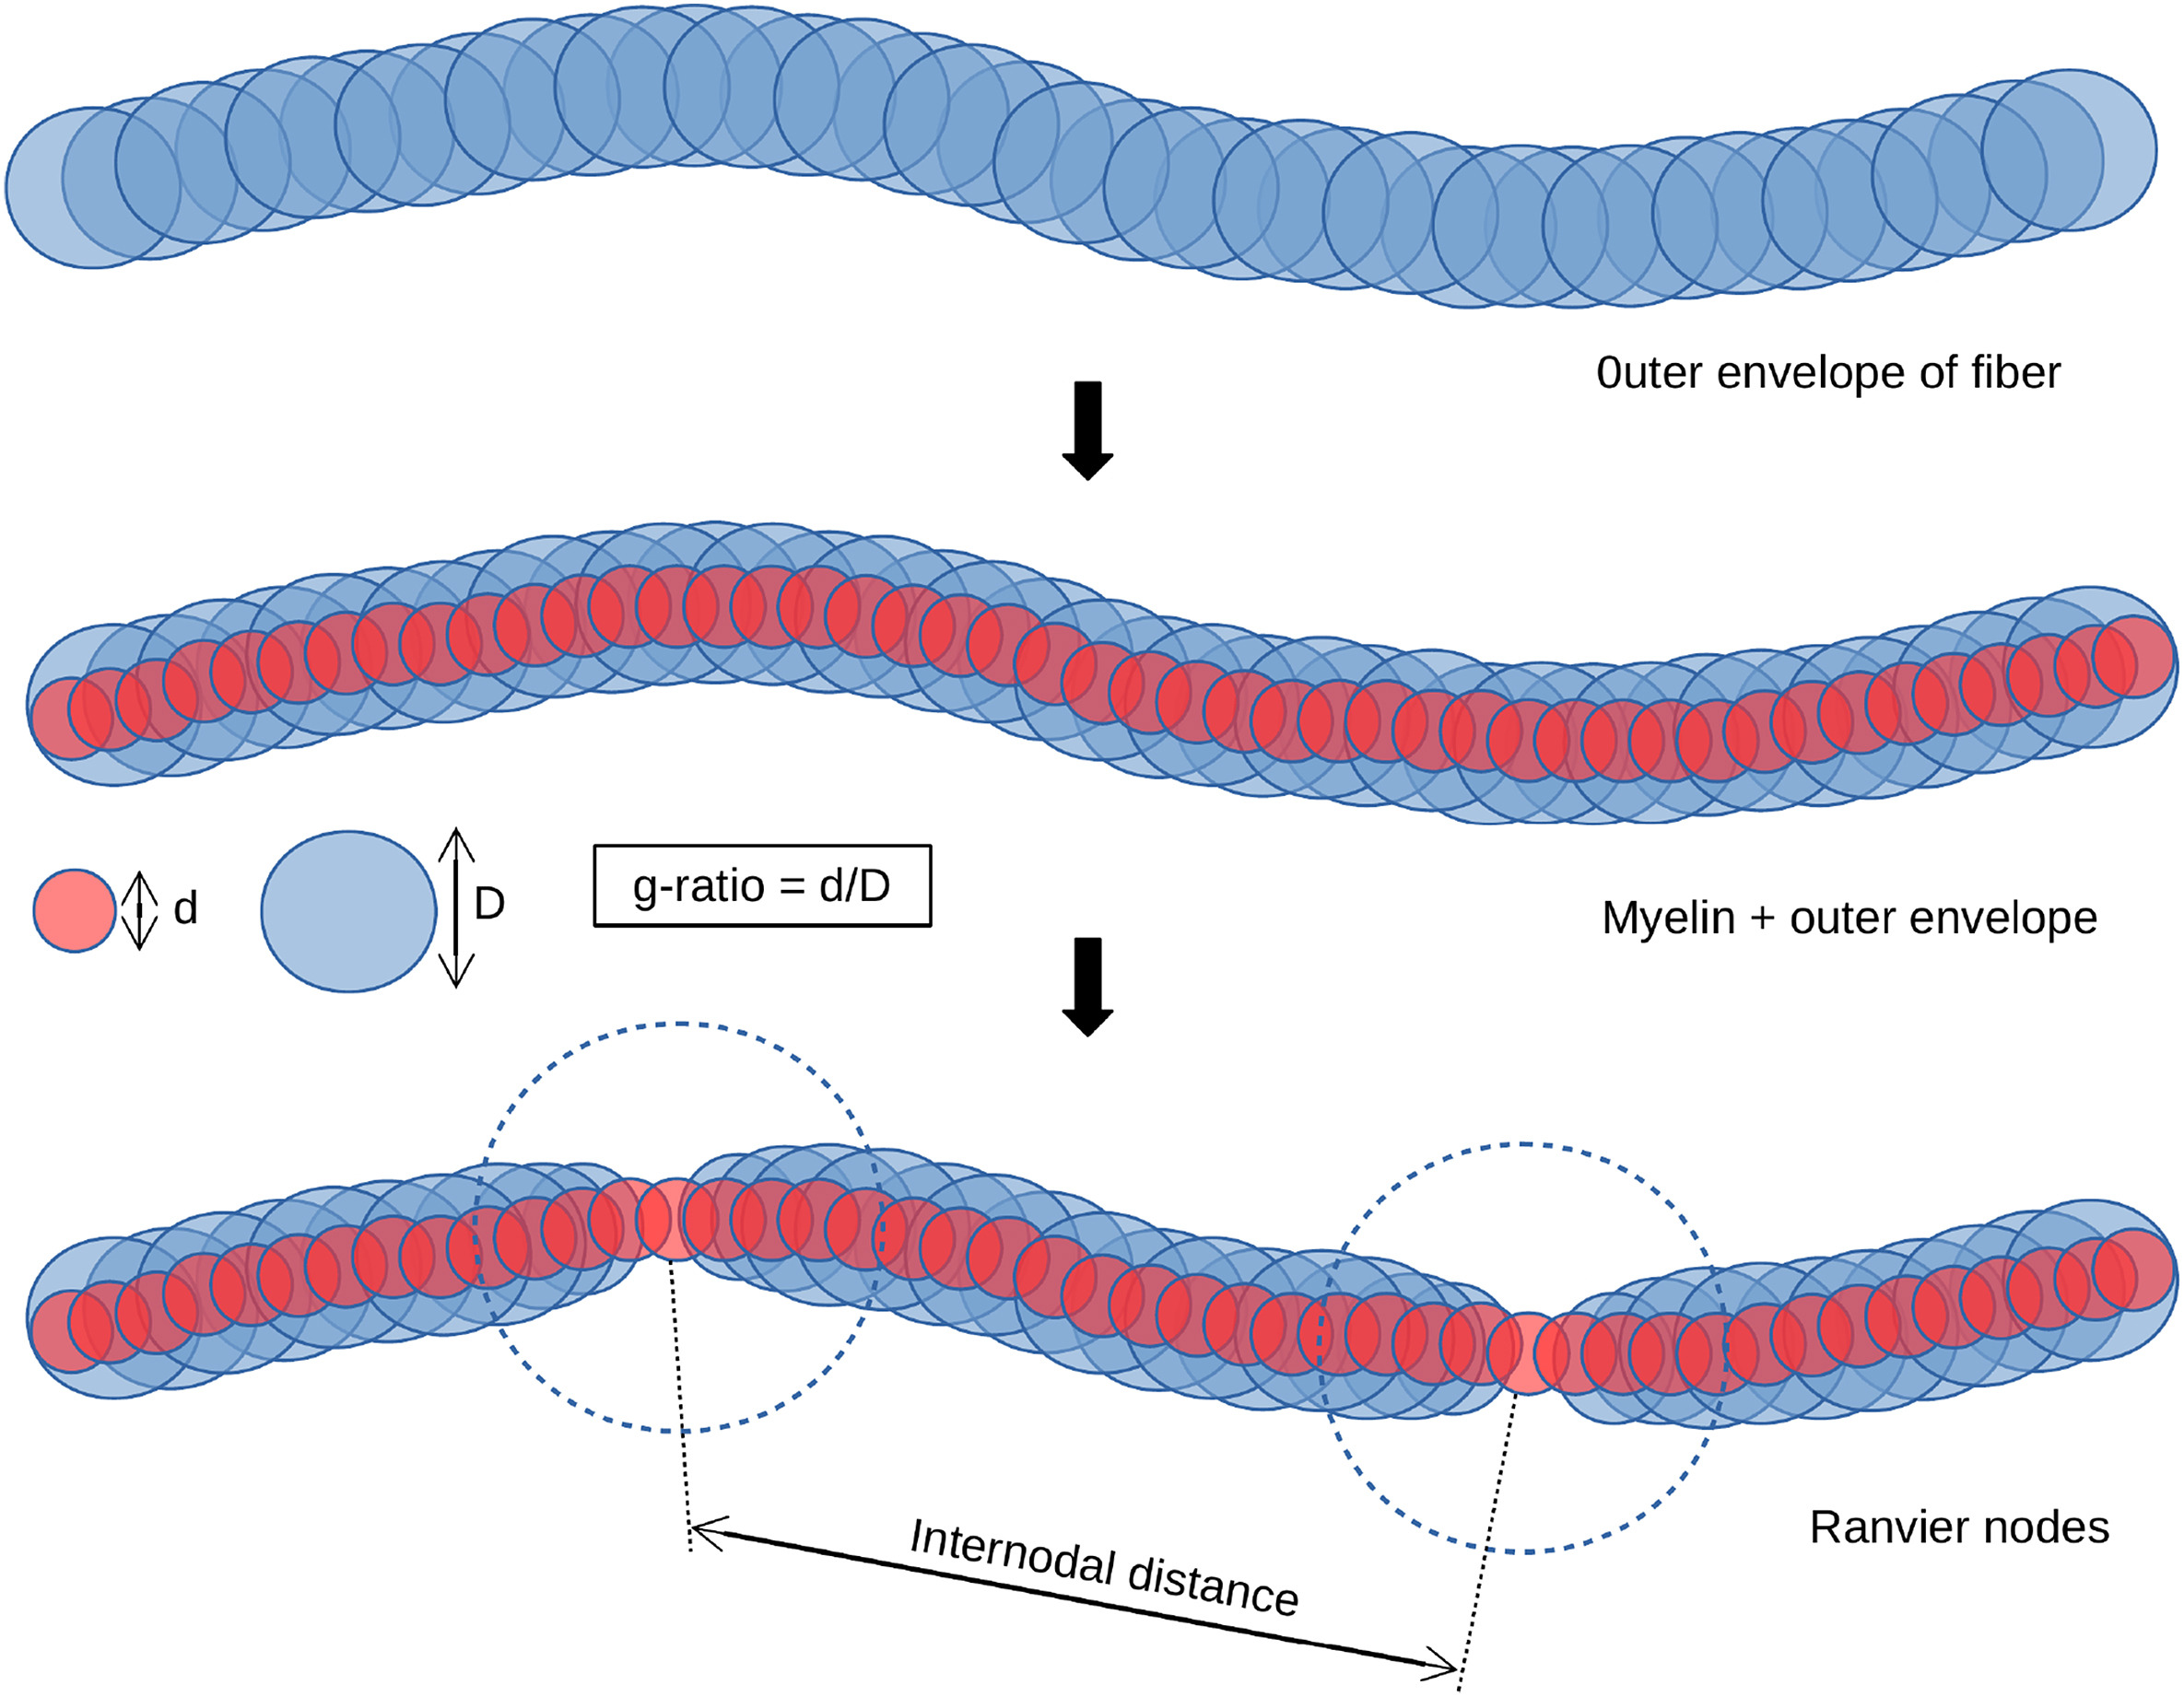
\includegraphics{gfx/model/medusa/4.jpg}
%     % }
% 	\caption{4 \cite{Ginsburger2019}}
% 	\label{fig:model:medusa_4_org}
% \end{figure}
% 
Since all objects are represented as a collection of spheres (see \cref{fig:model:medusa_4})
\begin{align}
    \mathcal{S} = \{ (x_i,y_i,z_i,r_i) : i \in \{0, 1, ..., n_\text{objects}-1\}  \} 
\end{align}
% 
, a collision is present if (VCS !!!)
% 
\begin{align}
\begin{split}
d<r_i+r_j\\
d = \abs{\vv{p}_i - \vv{p}_j}
\end{split}
\end{align}
% 
However since neighboring spheres in one fiber are colliding for a densly populated fiber, they have to be excluded if
\begin{align}
\begin{split}
d(i,j) &\leq  r_i + r_j\\
d(i,j) &= 
\begin{cases}
\sum_{n=i}^{j-1} \abs{\vv{p}_n - \vv{p}_{n+1}},& \text{if } j-i \geq 1\\
0 & \text{otherwise}
\end{cases}
\end{split}
\end{align}
% 
Spheres inside cell bodys are not checked for collision, since their volume aproximate? the volume of the cell.\\
% 
The calculation of collisions is done via the GPU architecture. For this a first implementation was written with the \textit{AxisAligedSortedSearch} \cite{Karras2012}. It sorteds the spheres along one axis, \eg x-axis, and search for each sphere the fist and last possible collision on this axis:
\begin{align}
\begin{split}
\mathcal{C}_i = \{ s \in \mathcal{S} \mid \abs{s_i.x - s_j.x} < r_i+r_j \}
\end{split}
\end{align}
% 
\begin{lstfloat}[!t]
	\lstinputlisting[style=cpp]{code/medusa.cu}
	\caption{Pseudocode of \acs{MEDUSA} collision checking.}
	\label{alg:medusa_collision}
\end{lstfloat}
% 
The above described algorithm is currently used for volumes $\approx \SI{200}{\micro\meter}$. For this volume size the algorithm is for the current use fast enough. However, more advaned algorithm exist wich can be applied here (\eg \textit{BoundindBoxHierarchy} \cite{Karras2012}).
% 
\begin{figure}[!t]
    \centering
    \resizebox{0.95\textwidth}{!}{
    \includegraphics{gfx/model/medusa/8.jpg}}
	\caption{8 \cite{Ginsburger2019}}
	\label{fig:medusa_8}
\end{figure}
% 
\begin{figure}[!t]
    \centering
    \resizebox{0.95\textwidth}{!}{
    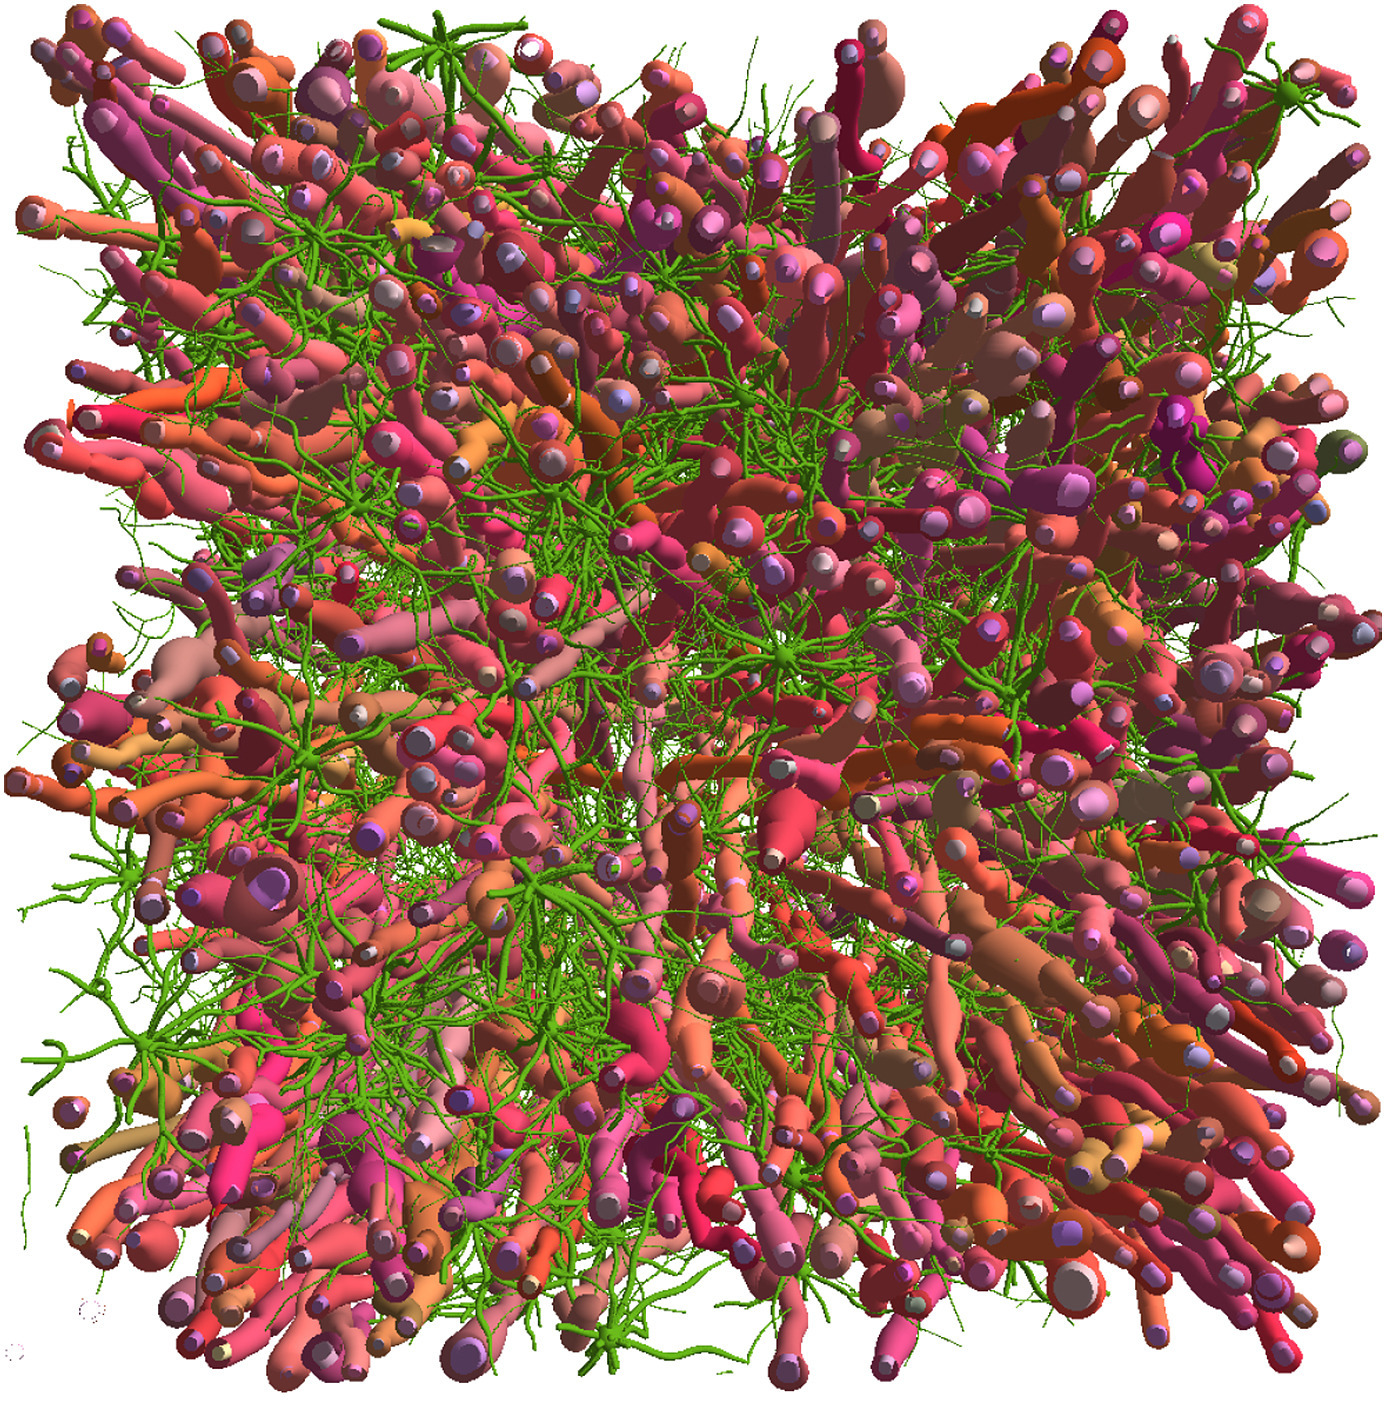
\includegraphics{gfx/model/medusa/11_.jpg}}
	\caption{11 \cite{Ginsburger2019}}
	\label{fig:medusa_11}
\end{figure}
% 
% 
% 
% 
% 
% 
% 
%
% Neurospin works with \ac{dMRI} signals.
% One focus is on the analysis of the fiber architect of the human brain.
% \ac{dMRI} is here quite handy since it is currently the only technique to allow in-vivo measurements to analyse the orientation of white matter tracts. Another importance is the availability of \ac{MRI} machines in almost every hospital in the western civilization.
% Although their resolution is with \SIrange{1.5}{3}{\tesla} limited.
% However, Neurospin is equipped with a mordern \SI{7}{\tesla} \ac{MRI}.
% This makes it possible, including higher measurments times on post mortem brain tissue, a \ac{dMRI} resolution up to \SI{200}{\micro\meter}.
% This makes it possible to allow \ac{3D-PLI} to verify and enhance the analysis of current developed tractography data. 
% %
% Along this works they developed a simulation tool (name) which is computing a Monte-Carlo simulation on the diffusion process in virtual tissues.
% Therefore, for simulations of the \ac{dMRI} signal in the brain, geometric models of nerve fibers as well as nerve cells are required.
% %
% The common goal was, due to a work packes inside the \ac{HBP}, the development of a common general purpose tool to build a geometrical library of nerve fiber configurations.
% Therefore it was decided to work based on the first approaches \cite{Ginsburger2018}.
% %
% \begin{quotation}
% We design a novel white matter numerical phantom generation algorithm which constructs biomimicking geometric configurations with few design parameters, and enables to control the level of disorder of the generated phantoms. The influence of various geometrical parameters present in white matter, such as global angular dispersion, tortuosity, presence of Ranvier nodes, beading, ...
% \end{quotation}
% %
% It is therefore qualified to generate a large database or library of parameter controlled white matter volumes.
% %
% \paragraph{differences:} 
% \begin{itemize}
%     \item All objects are aproximated with spheres.
%     \item Statistical ... of tissue
%     \item diffusion specific parameters
%     \item pathological changes like axon beeding
% \end{itemize}
% 
\section{"Conclusion"}
This allows a user to specify any initial configuration and reaching a collision free model, which, depending on the initial overlap, follows the initial geometry.
The disadvantage obvious is that the configuration has to change.
However since biological tissue is deformable and not "caotic" itself, it follows its natrual behavier.